\textbf{Motivation.} Here is the motivation.

\textbf{Diffie-Hellman key exchange.} Diffie-Hellman protocol is a method of asymmetric exchange of secrets for
a group of two or more participants,
developed in 1976 by cryptographers Ralph Merkle and Whitfield Diffie and Martin Hellman.
In contrast to symmetric key exchange, the diffie-hellman protocol eliminates the direct transfer of the shared secret.
between participants, each participant computes a shared secret with its own private / public key pair.
The Diffie Hellman protocol is based on a one-way function of the form

\[
    A = G ^ a mod P,
\]

where A is the user's public key, a is the user's private key, P is modulus, which is at least 2048 bit prime,
G - primitive root modulo P.

Thus, the safety of the Diffie-Hellman protocol is based on the discrete logarithm problem, which is unsolvable
in polynomial time if the constants G and P are chosen correctly.
Graphically, the essence of the Diffie Hellman protocol can be expressed through the analogy with mixing paints, as shown in
image below
\begin{figure}[H]
    \centering
    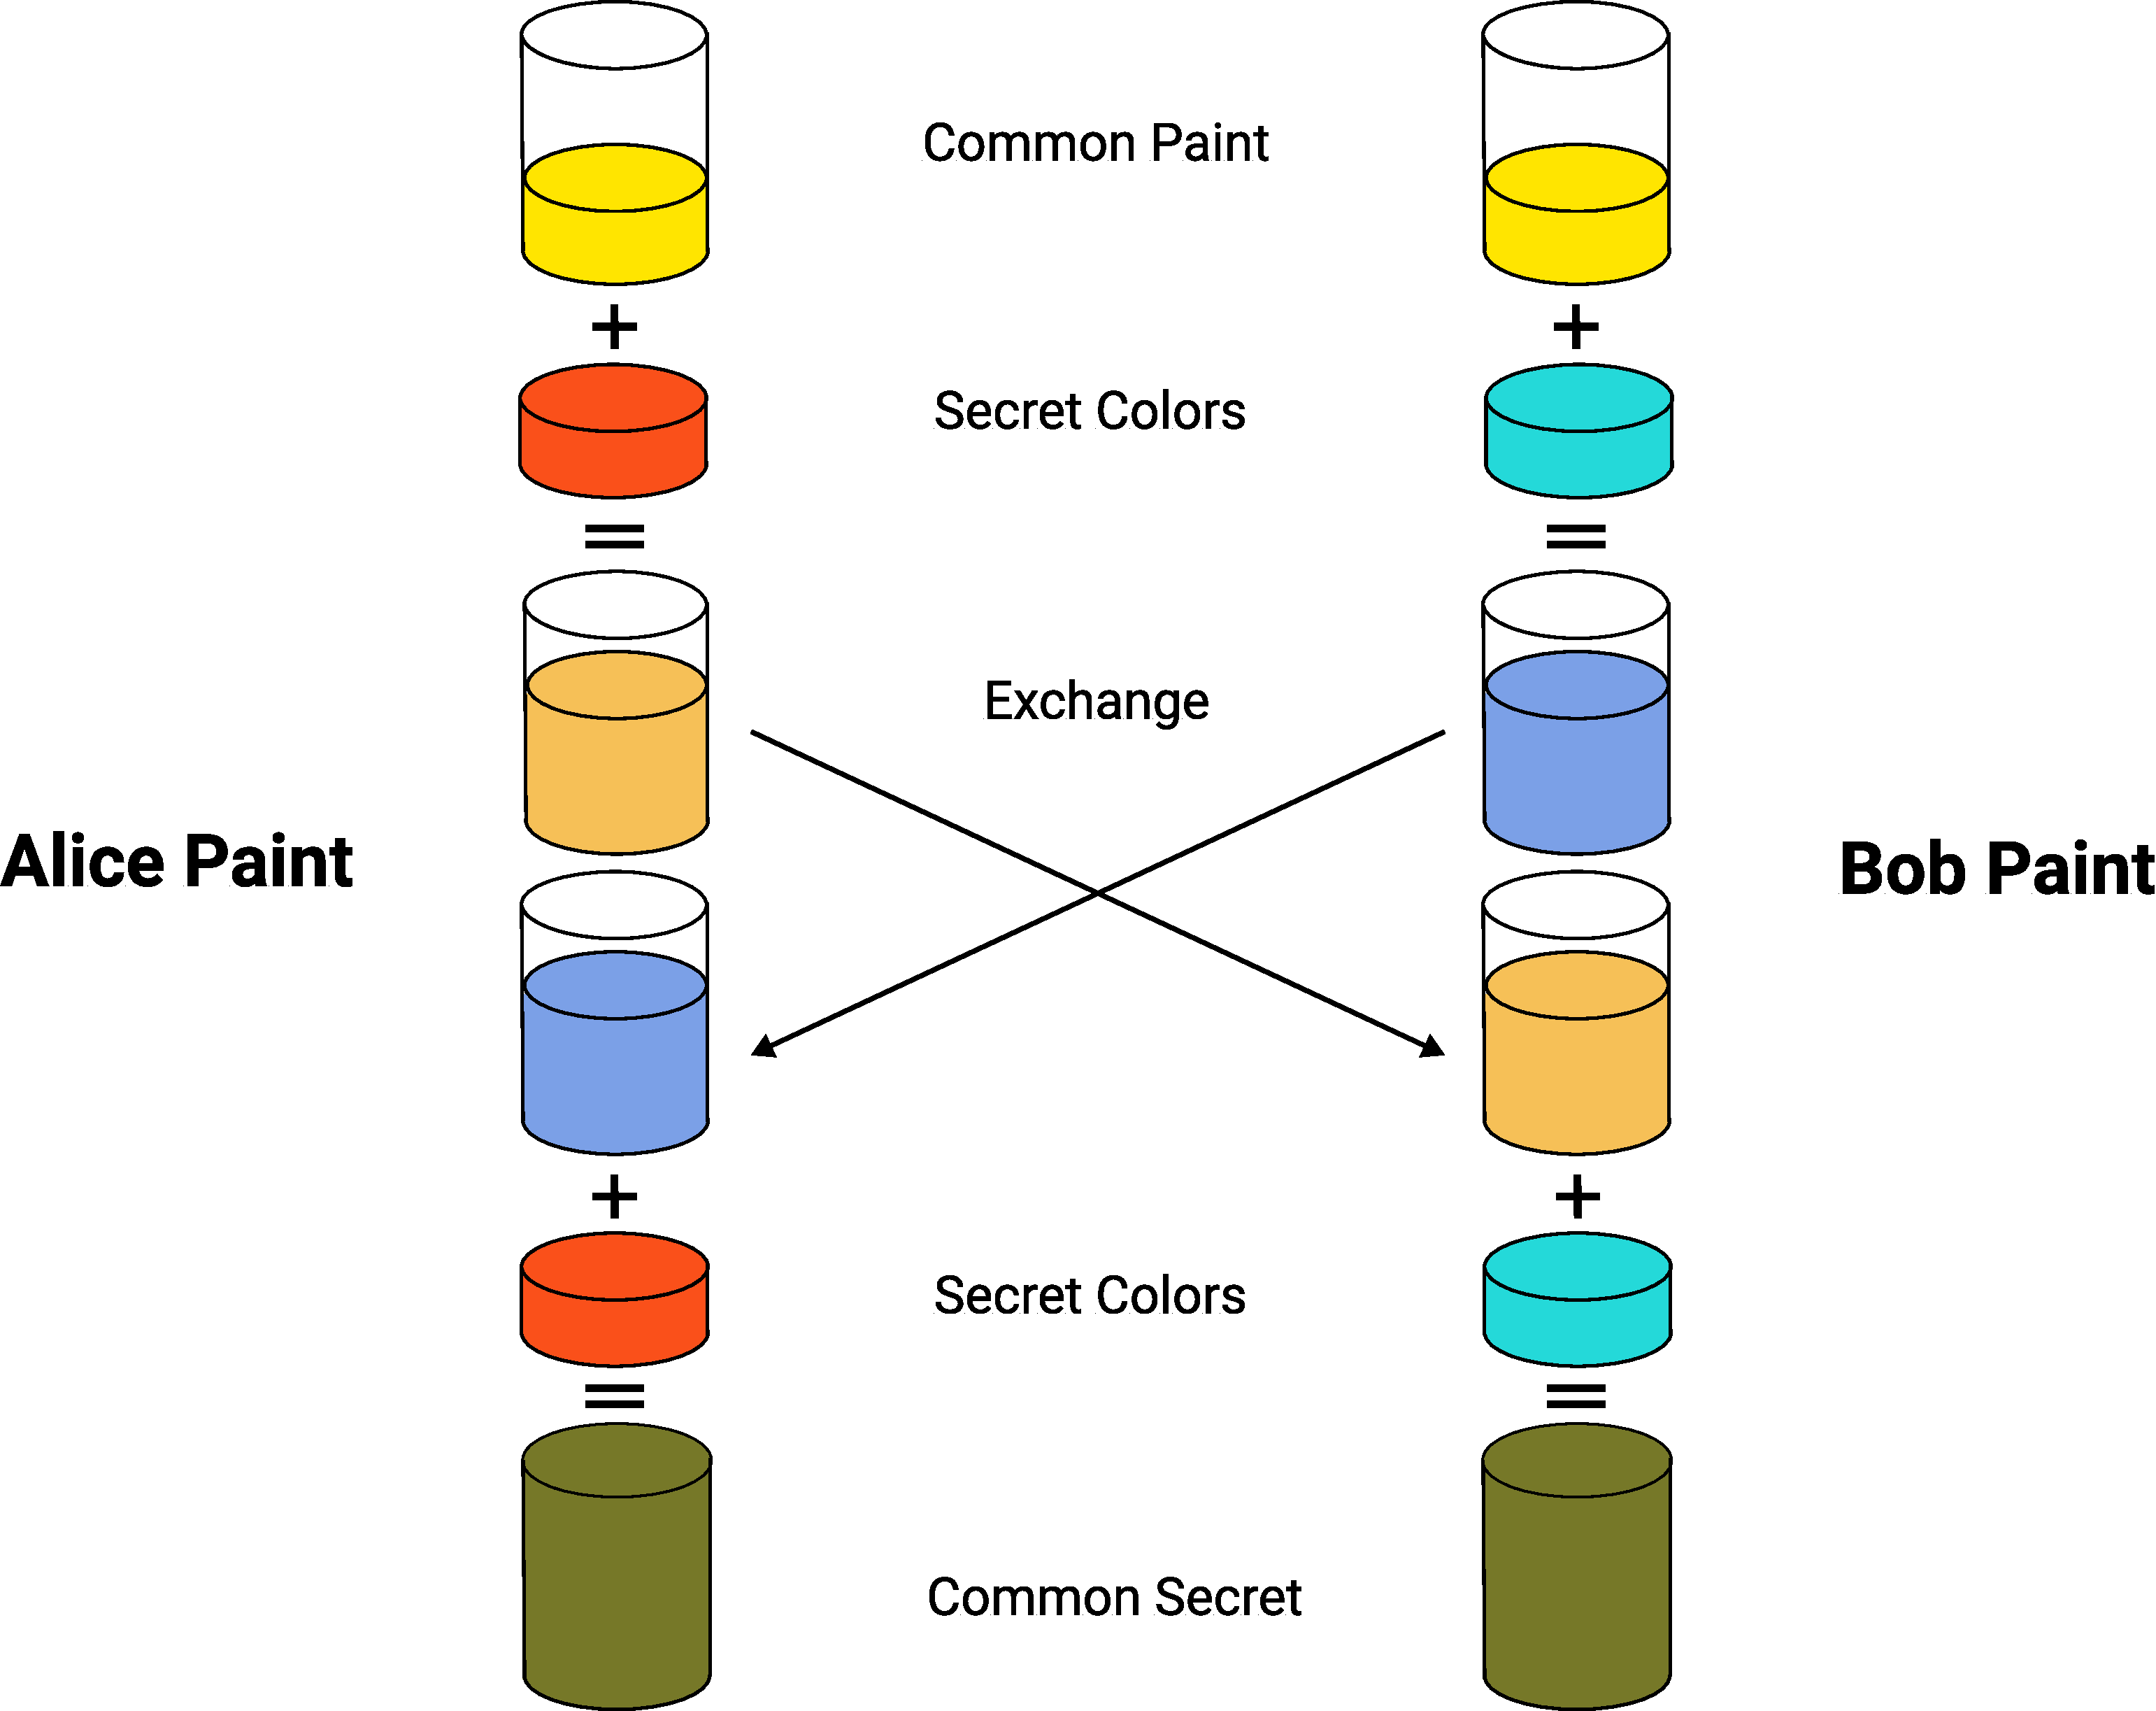
\includegraphics[width=1\textwidth]{Pictures/Diffie-Hellman}
    \caption{Illustration of the concept behind Diffie–Hellman key exchange. Source: }\label{fig:figure4}
\end{figure}
In contrast to the diffie-hellman based on discrete logarithm problem, there is an elliptic curve diffie hellman
key exchange, which based on the elliptic curve discrete logarithm problem.
Although, the idea is quite same, but elliptic curve diffie hellman ensures the same safety as discrete logarithm
diffie-hellman with lesser value of the modulus P.
For instance, 521 bit modulus used in elliptic curve diffie hellman is equally safe as 2048 bit modulus in
discrete logarithm diffie-hellman.
To summarize, the flow of diffie hellman kay exchange is as follows
\begin{enumerate}
    \item Given modulus $P$ and generator $G$.
    \item Alice chooses her secret $a$.
    \item Alice sends to Bob $A, \; A = G^a \bmod P$.
    \item Bob chooses his secret $b$.
    \item Bob sends to Alice $B, \; B = G^b \bmod P$.
    \item Alice computes common secret $s, \; s = B^a \bmod P = (G^b \bmod P)^a \bmod P$.
    \item Bob computes common secret $s, \; s = A^b \bmod P = (G^a \bmod P)^b \bmod P$.
    \item Alice and Bob have arrived to the same value
    \[
        A^b \bmod P = G^{ab} \bmod P = G^{ba} \bmod P = B^a \bmod P,
    \]
    more specially,
    \[
        (G^a \bmod P)^b \bmod P = (G^b \bmod P)^a
    \]
\end{enumerate}

%\begin{figure}[H]
%    \centering
%    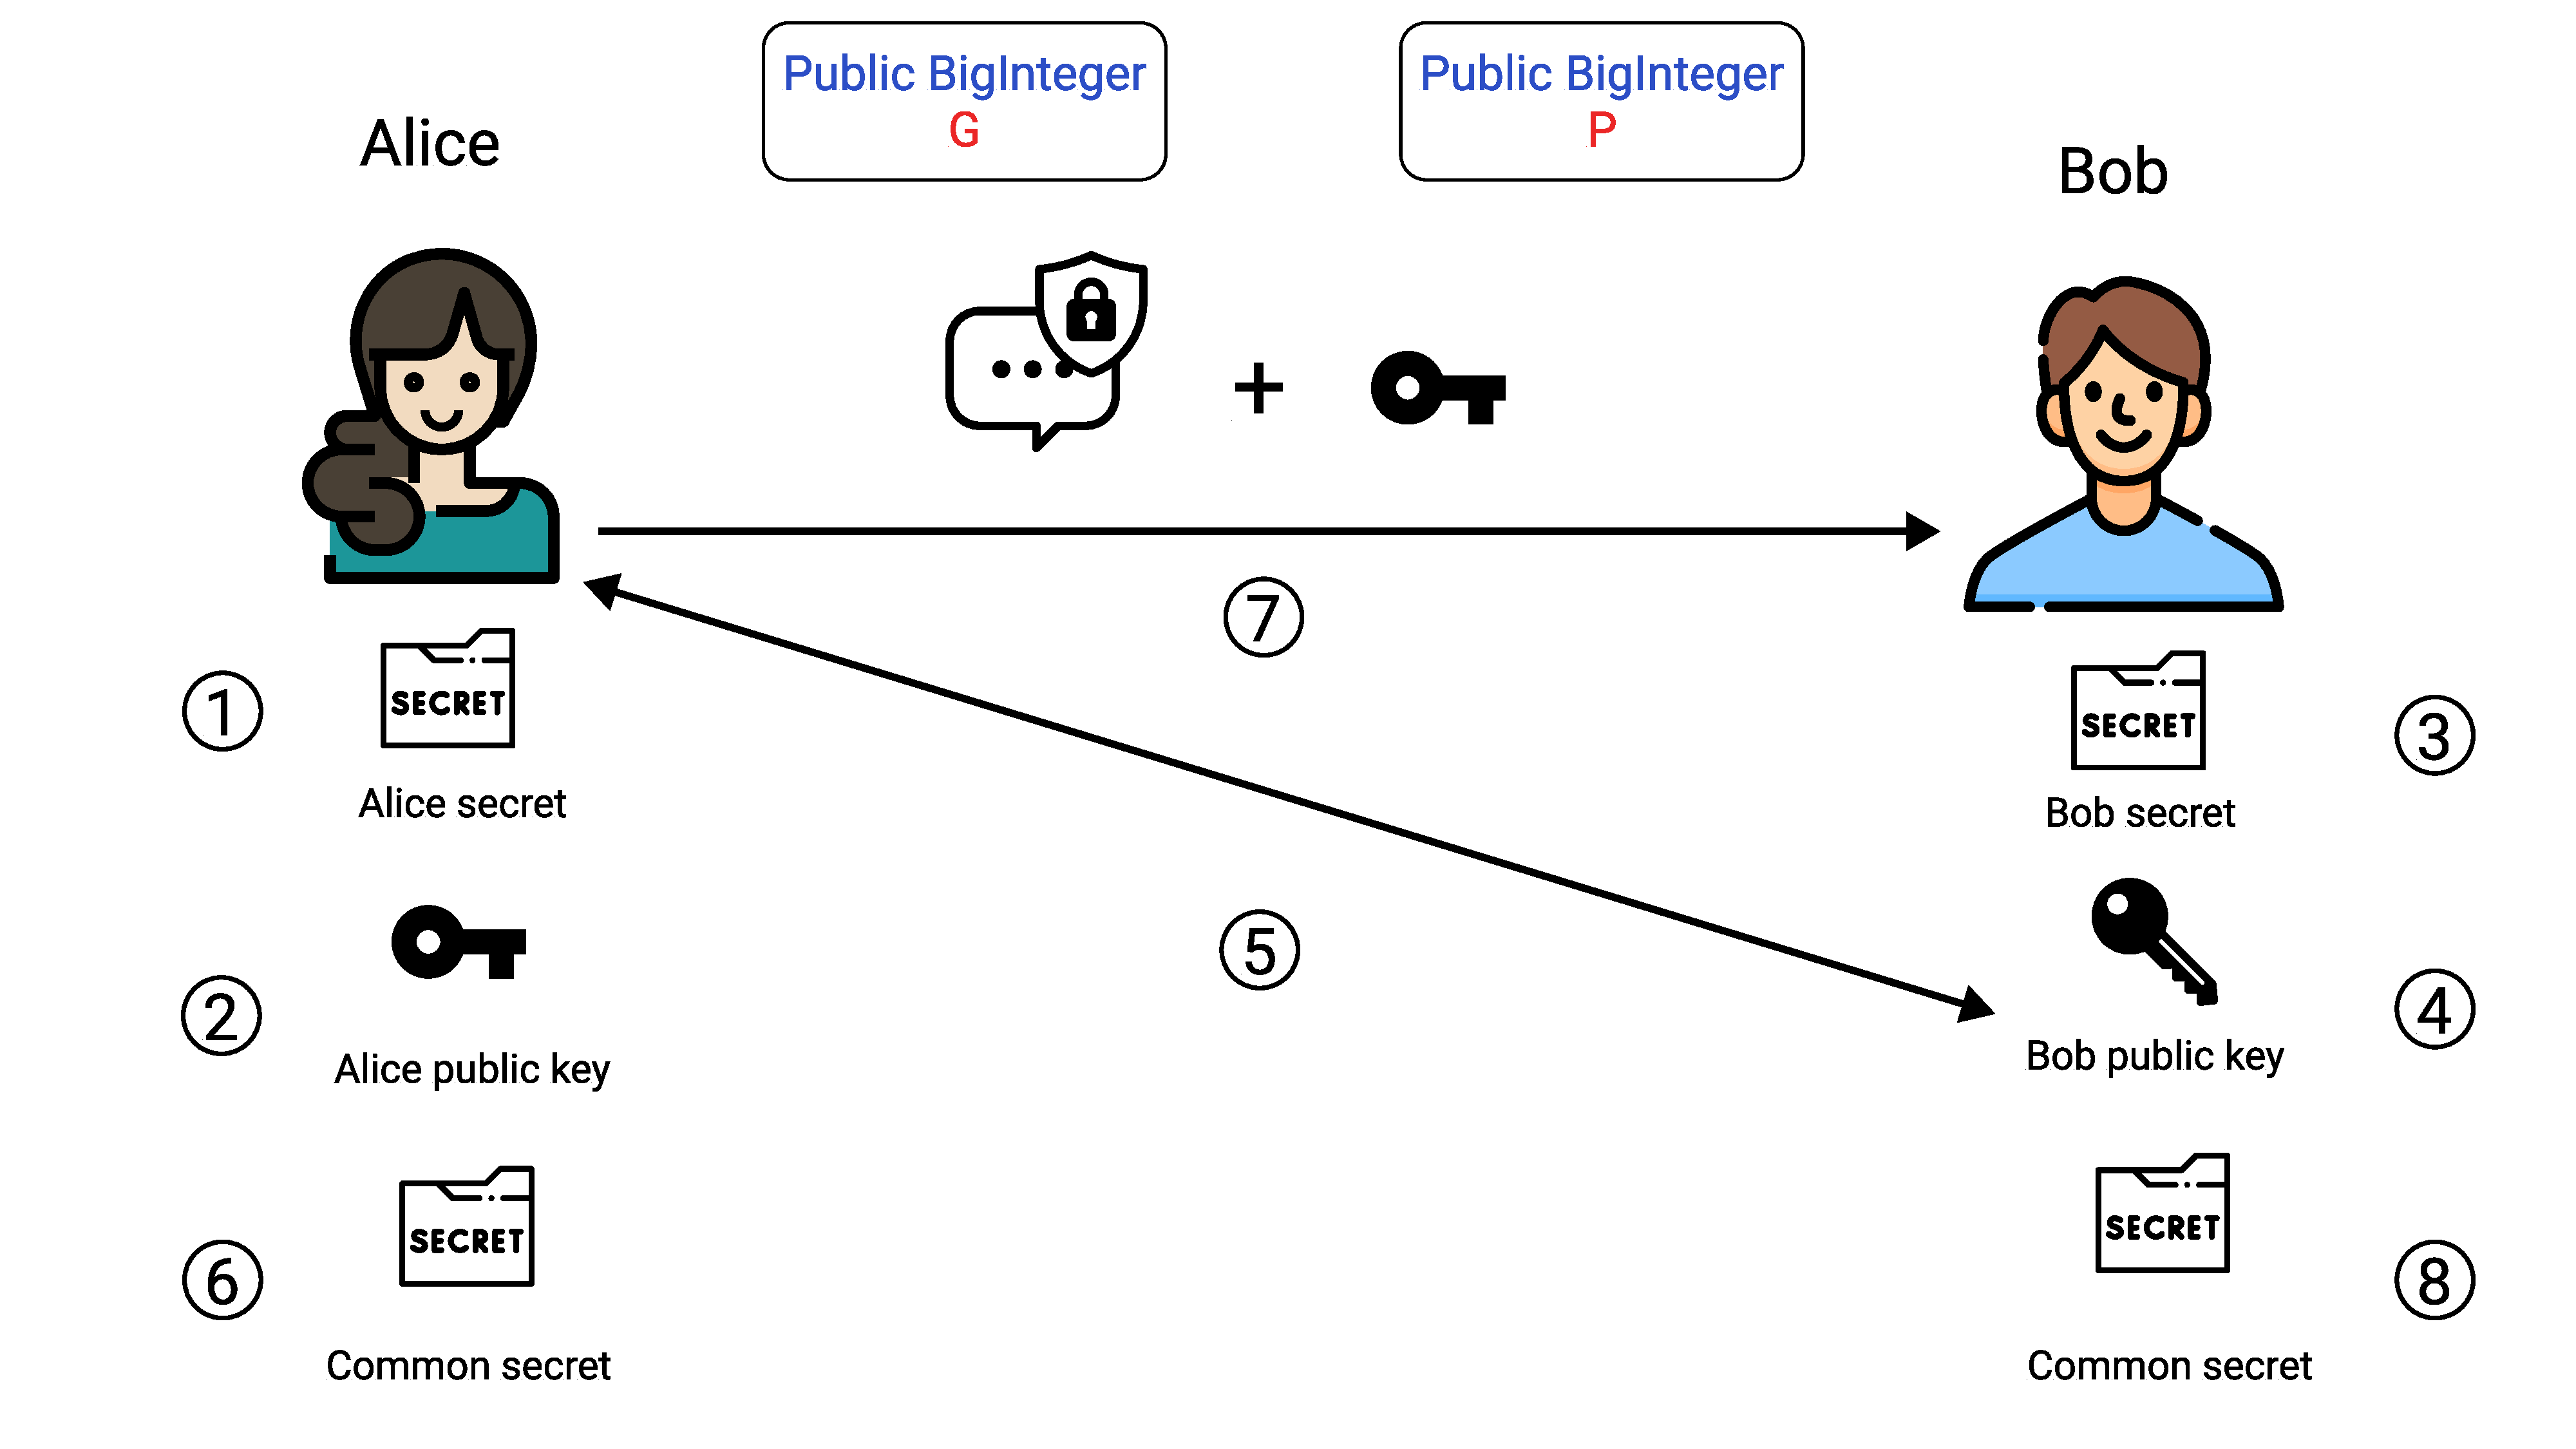
\includegraphics[width=1\textwidth]{Pictures/Key_Exchange}
%    \caption{Secret chat encryption concept diagram. Source: }\label{fig:figure7}
%\end{figure}